\documentclass{article}
\usepackage[UTF8]{ctex}  % 使用中文支持包
\usepackage[a4paper, margin=1in]{geometry}  % 设置纸张大小和边距
\usepackage{anyfontsize}  % 解决字体大小报错问题
\usepackage{fancyhdr}  % 设置页眉、页脚、页码
\usepackage{longtable}  % 支持长表格

\usepackage{amsmath}  % 数学公式支持
\usepackage{cases}  % 支持联立编号
\usepackage{cite}  % 引用支持

\usepackage{graphicx}  % 插入图片支持
\usepackage{float}  % 设置图片浮动位置
\usepackage{subfigure}  % 插入多图时用子图显示

\usepackage{listings}  % 代码块支持
\usepackage{xcolor}  % 设置代码块颜色

\usepackage[hyphens]{url}  % 支持链接换行
\usepackage{hyperref}  % 超链接支持
\usepackage{lastpage}  % 添加lastpage包

\usepackage{gbt7714}  %国标参考文献

\hypersetup{
    hidelinks,
    colorlinks=true,
    allcolors=black,
    pdfstartview=Fit,
    breaklinks=true
}

\title{聚变能源概论-第四讲作业}
\author{\LaTeX\ by\ 何宇峰\ }
\date{\today}
\pagenumbering{arabic}

\begin{document}
\pagestyle{fancy}

\fancyhead[L]{何宇峰}
\fancyhead[C]{聚变能源概论-第四讲作业}
\fancyhead[R]{\today}
\fancyfoot[C]{Page \thepage/\pageref{LastPage}}

\section{劳逊判据曲线绘制}
\emph{不同的热电效率对应不同的劳逊判据, 请分别画出 $\eta = 0.3$ 和 $0.5$ 时 $n\tau E$ 对 $T$ 的曲线, 并在同一个图中画出点火条件, 说明点火条件相当于 $\eta$ 等于多少时的劳逊判据. }

$n\tau_E$ 与 $T$ 的关系如下:

$$n_{\tau_E} \geq \frac{3T(1 - \eta)}{\left[\frac{1}{5} + \frac{4}{5}\eta\right]\frac{1}{4}\langle \sigma v \rangle_{DT} E_{DT} - (1 - \eta) C_B \sqrt{T}}$$

取$E_{DT} = 17.6 \text{MeV}$, $C_B = 5.355 \times 10^{-37}$, $\eta = 0.3$ 或 $0.5$, 代入上式, 结合$\langle \sigma v \rangle_{DT}$ 与 $T$ 的关系式, 可得 $n\tau E$ 与 $T$ 的关系曲线.

\begin{figure}[htpb]
    \centering
    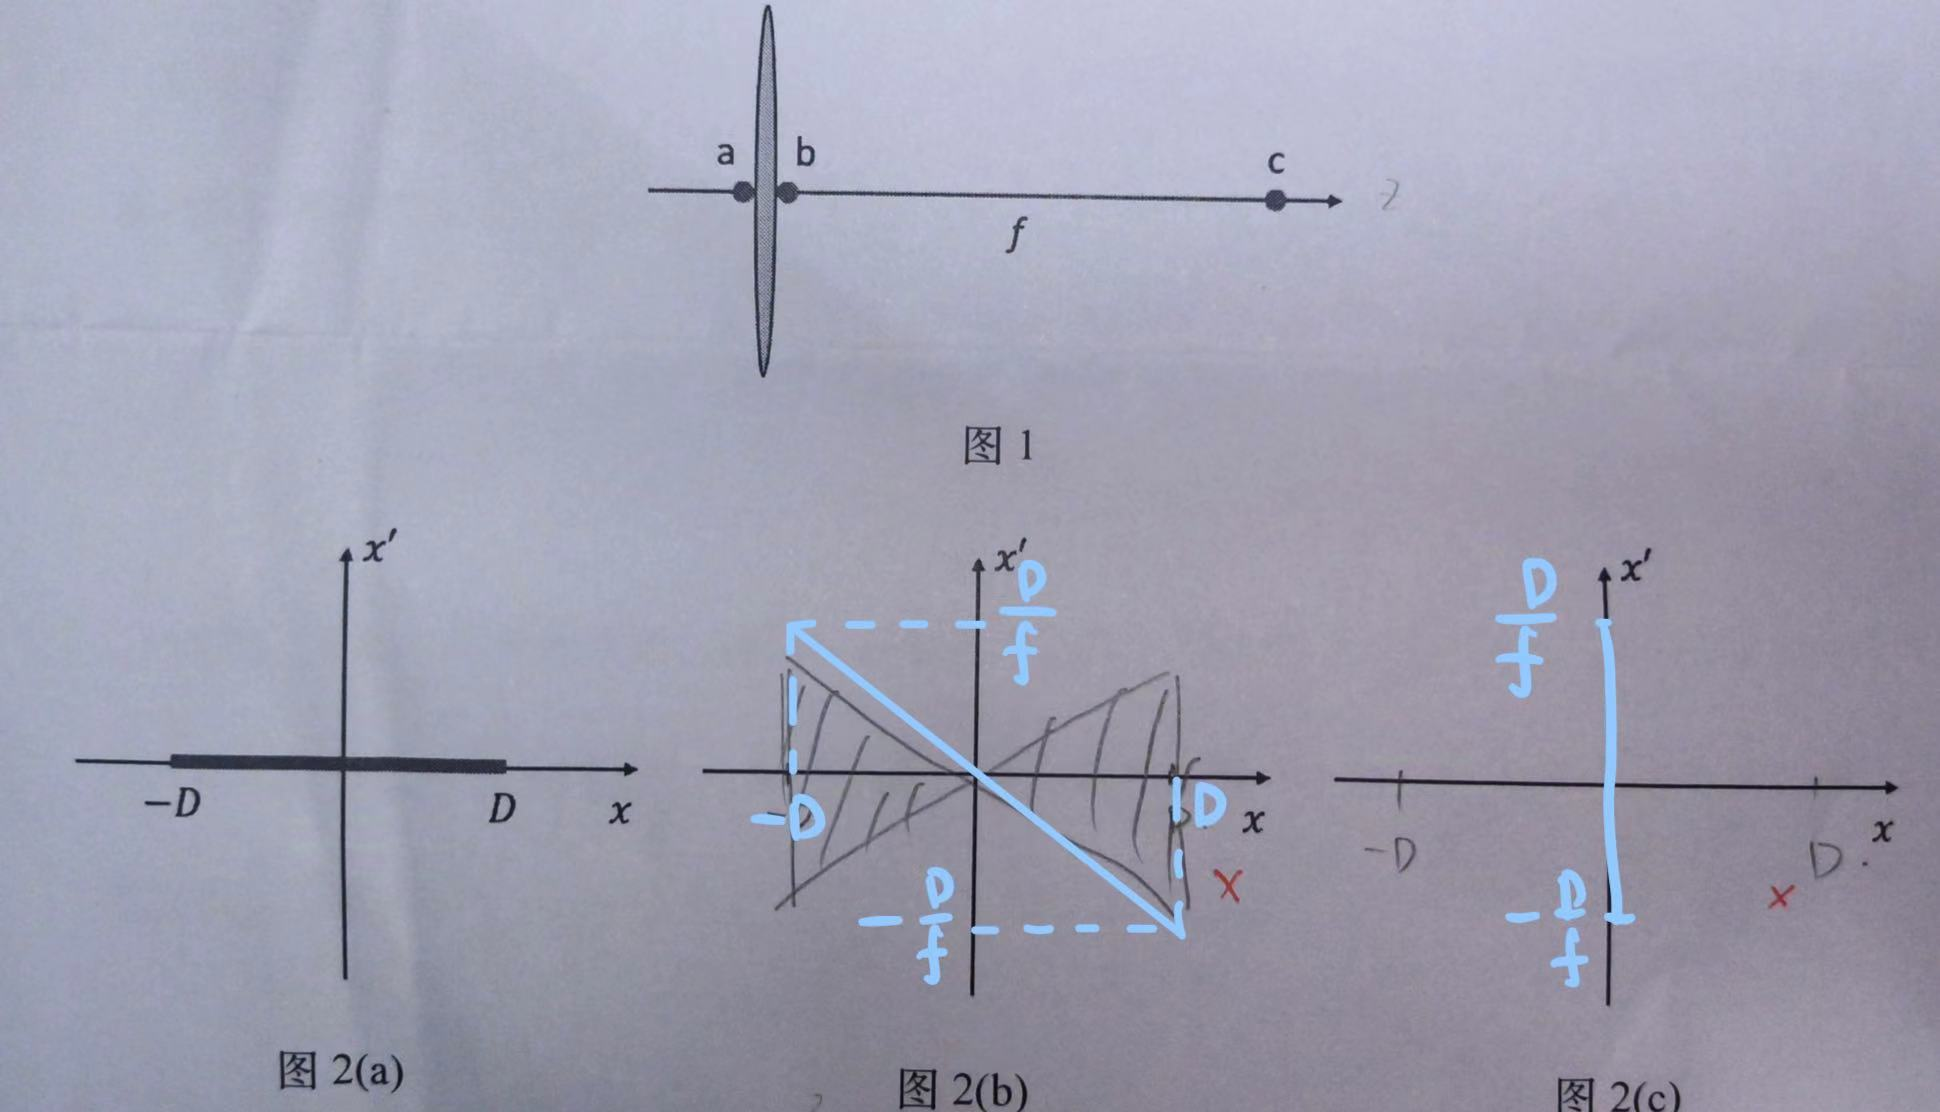
\includegraphics[width=0.8\textwidth]{img/1.pdf}
    \caption{Lawson 判据曲线}
    \label{fig:1}
\end{figure}

\section{点火条件计算}
\emph{对于不含催化反应的 D-D 聚变、半催化的 D-D 聚变、完全催化的 D-D 聚变, 分别计算其点火条件. }

DD反应由反应截面近似相等的反应道组成:

$$\text{D} + \text{D} \rightarrow \text{He}^3 + \text{n} + 3.267 \text{MeV}$$
$$\text{D} + \text{D} \rightarrow \text{T} + \text{p} + 4.032 \text{MeV}$$

所谓半催化和完全催化指的是考虑DT反应和D-He3反应之后的后果:

$$ 5\text{D} \rightarrow 2n + p + \alpha + 24.9 \text{MeV} (\text{半催化})$$
$$ 6\text{D} \rightarrow 2n + 2p + 2\alpha + 43.2 \text{MeV} (\text{完全催化})$$

所以区别只在放能和带电粒子的占比。

\begin{table}[htpb]
    \centering
    \label{tab:reactions-and-energy}
    \begin{tabular}{|l|c|c|}
    \hline
    反应类型 & 一对粒子放能 $E_f$/MeV & 产物带电粒子能量占比 $k$ \\ \hline
    无催化 & 3.6 & 0.67 \\ \hline
    半催化 & 10.0 & 0.34 \\ \hline
    完全催化 & 14.4 & 0.62 \\ \hline
    \end{tabular}
    \caption{不同反应的放能和带电粒子能量占比}
\end{table}

将这些式子代入点火条件的表达式($r_1=0.5$, $r_2=3$)

$$n_{\tau _{\mathrm{E}}} \geq \frac { r_2 T(1-\eta ) } { [k+(1-k)\eta ]r_1 \langle \sigma v \rangle E_f -(1-\eta )C_B Z_{eff}\sqrt{T}}$$

画图得到点火条件。

\begin{figure}[htpb]
    \centering
    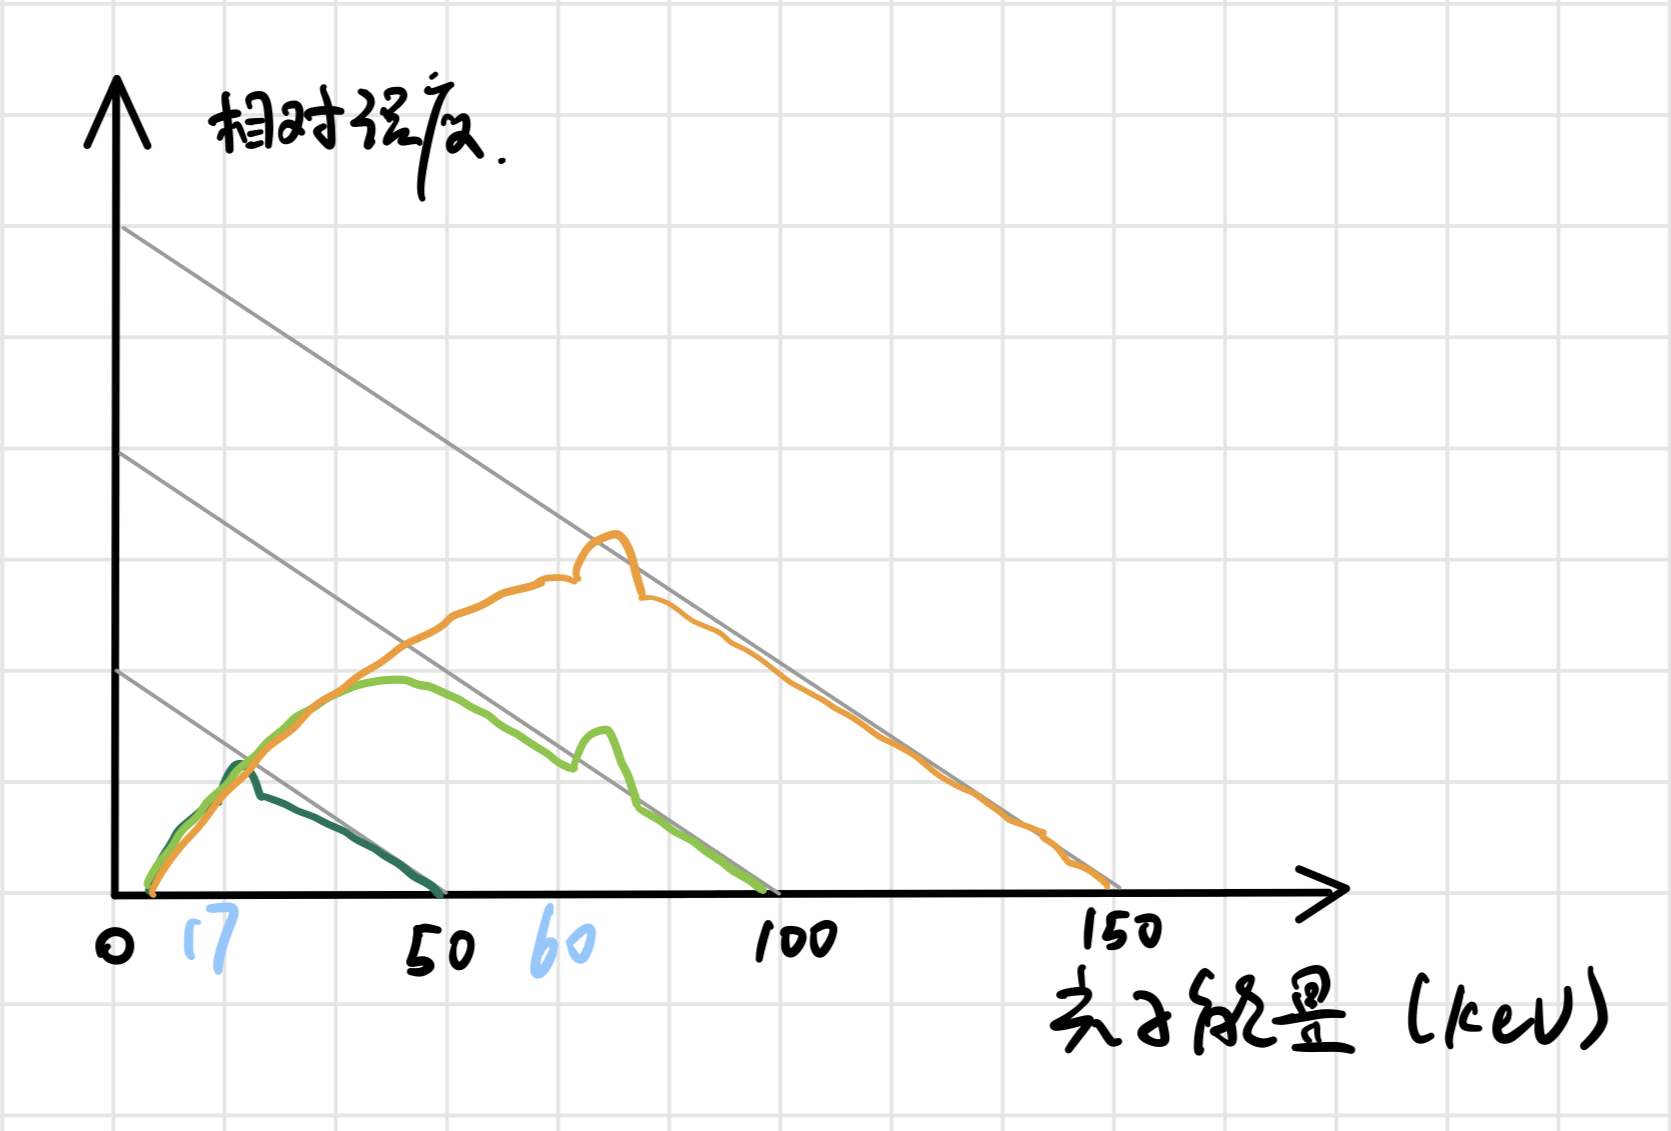
\includegraphics[width=0.8\textwidth]{img/2.pdf}
    \caption{点火条件计算}
    \label{fig:2}
\end{figure}

\section{D-T 聚变反应堆功率计算}
\emph{假设一个 D-T 聚变反应堆工作在密度 $4 \times 10^{19} \, \text{m}^{-3}$, 离子温度 10 keV, 能量约束时间 5 s, 外部加热功率为 50 MW 的状态, 请计算:}
\begin{enumerate}
    \item \emph{该聚变堆输出的净热功率及净电功率(按照 40\% 的热电转换效率, 70\% 电能到加热功率的转换效率、70\% 的有效加热功率计算); }
    \item \emph{等离子体密度极大地影响着聚变堆的运行参数. 假如等离子体密度在原有水平上提高了 20\%, 计算此时聚变堆输出的净热功率及净电功率. }
\end{enumerate}

\textbf{1. 计算过程如下:}

D-T聚变反应功率$S_f = \frac{1}{4} n_e^2 \langle \sigma v \rangle E_f = 1.277 \times 10^5 \text{W}/\text{m}^3$

轫致辐射功率$S_B = 5.139\times 10^{-37} n_e^2 \sqrt{T_i} = 2600\text{W}/\text{m}^3$

热传导功率$S_C = 3n_e k T_i \frac{d T_i}{d t} = 1.5 \times 10^5 \text{W}/\text{m}^3$

体系消耗功率密度$S_{h,ext}=S_\kappa +S_B -\frac{S_f}{5}$

外部输入热功率$P_{in} = 50\text{MW}$

外部输入电功率$P_in^{(E)} = \frac{1}{\eta_e\eta_a}S_{h,ext}V$

输出热功率是氚增殖热功率

$$P_{out}^{(H)} = \left[ \left( 1 + k_T \right)^4 S_f + S_\kappa + S_B + \frac{1 - \eta_a}{\eta_a} S_{h,ext} \right] V$$

输出电功率是输出热能转电效率

$$P_{out}^{(E)} = \left[ \left( 1 + k_T \right)^4 S_f + S_\kappa + S_B + \frac{1 - \eta_a}{\eta_a} S_{h,ext} \right] V $$

有

$$P_{in}^{(E)} = \frac{1}{\eta_e \eta_a} S_{h,ext} V \Rightarrow P_{in}^{(H)} = \frac{1}{\eta_a} S_{h,ext} V$$

故

$$V = \frac{P_{in}^{(H)} \eta_a}{S_\kappa + S_B - S_f/5} = 2263.91 \text{m}^3$$

净输出热功率

\begin{equation*}
    \begin{aligned}
        P_{out}^{(H)} - P_{in}^{(H)}
        &= \left[ (1 + k_T)^4 \frac{S_f}{5} S_\kappa + S_B + \frac{1 - \eta_a}{\eta_a} S_{h,\text{ext}} \right] V - P_{in}^{(H)} \\
        &= \left[ (1 + k_T)^4 \frac{4}{5} + \frac{1}{5} \right] S_f V \\
        &= 367.83 \text{MW}
    \end{aligned}
\end{equation*}

净输出电功率

\begin{equation*}
    \begin{aligned}
        P_{o u t}^{(E)} - P_{i n}^{(E)}
        &= \eta\left[(1+k_T)^4 \frac{S_f}{5} + S_\kappa + S_B + \frac{1-\eta_a}{\eta_a} S_{h, e x t}\right] V - \frac{1}{\eta_e} P_{i n}^{(H)} \\
        & = \eta\left[(1+k_T)^4 \frac{S_f}{5} + S_\kappa + S_B + \left(\frac{1-\eta_a}{\eta_a} - \frac{1}{m \eta_e \eta_a}\right) S_{h, e x t}\right] V \\
        &= 95.7 M W
    \end{aligned}
\end{equation*}

\textbf{2. 计算过程如下:}

密度提高$20\%$后, $n_e = 4.8 \times 10^{19} \text{m}^{-3}$, 重复上述计算, 得到

D-T聚变反应功率$S_f = 1.84 \times 10^5 \text{W}/\text{m}^3$

轫致辐射功率$S_B = 3.74 \times 10^3 \text{W}/\text{m}^3$

热传导功率$S_\kappa = 4.61 \times 10^4 \text{W}/\text{m}^3$

$V = 2.685 \times 10^3 \text{m}^3$

净输出热功率$P_{out}^{(H)} - P_{in}^{(H)} = 628.1 \text{MW}$

净输出电功率$P_{out}^{(E)} - P_{in}^{(E)} = 199.8 \text{MW}$

\section{工程增益因子解析关系式}
\emph{假定 alpha 粒子功率只有一小部分能量份额 $k$ 沉积在等离子体中, 其余的 $1 - k$ 流向第一壁并转化为热量. 不计 T 增殖产生的热量. 在典型效率: $\eta = 40\%$, $\eta_e = 70\%$, $\eta_a = 70\%$ 下, 推导工程增益因子 $Q_E$ 与 $k$ 及等离子体参数 $n\tau E T_i$ 的解析关系式, 并分别画出 $k = 0$, $0.5$, $1$ 时 $Q_E$ 对 $n\tau E T_i$ 的曲线. }

当$\alpha$粒子全都留在等离子体内时,$Q_E$的表达式为

$$Q_E = \frac{\eta\left(\left(1 - \frac{k}{5}\right)S_f + S_B + S_k\right)}{S_B + S_k - \frac{k}{5}S_f} - 1$$

考虑$S_B\rightarrow0, \frac{S_f}{S_\kappa}=5\cdot\frac{F}{F_i}$

有

$$Q_E = 0.98\cdot\frac{\frac{F}{F_I}}{1-k\frac{F}{F_I}} - 0.72$$

绘图如下:

\begin{figure}[htpb]
    \centering
    \includegraphics[width=0.8\textwidth]{img/4.pdf}
    \caption{$Q_E$ vs. $n\tau E T_i$}
    \label{fig:4}
\end{figure}

\end{document}
